% file thesis.tex
% Archivo thesis.tex
% Documento maestro que incluye todos los paquetes necesarios para el documento
% principal.

% Documento obtenido por un sinfin de iteraciones de administradores del LDC
% Estructura actual hecha por:
% Jairo Lopez <jairo@ldc.usb.ve>
% Actualizado ligeramente por:
% Alexander Tough 
% Actualizado con una estructura de carpetas por:
% Tony Lattke

\documentclass[oneside,12pt,letterpaper]{report}
\tolerance=1000  
\hbadness=10000  
\raggedbottom

% Para escribir algoritmos
\usepackage{listings}
\usepackage{algpseudocode}
\usepackage{algorithmicx}
\usepackage{algorithm}

% Paquetes para manejar graficos
\usepackage{epsf}
\usepackage[pdftex]{graphicx}
\usepackage{epsfig}
% Simbolos matematicos
\usepackage{latexsym,amssymb}
% Paquetes para presentar una tesis decente.
\usepackage{setspace,cite} % Doble espacio para texto, espacio singular para
                           % los caption y pie de pagina
\usepackage[table]{xcolor}
\usepackage{tikz}
\usetikzlibrary{shapes.geometric,arrows}

\usetikzlibrary{arrows,shapes}
\usepackage{verbatim}

\usepackage{comment}

% Paquetes no utilizados para citas
%\usepackage{mcite} 
%\usepackage{draft} 

\usepackage{wrapfig}
\usepackage{alltt}

% Acentos 
\usepackage[spanish,activeacute,es-noquoting]{babel}

\usepackage[spanish]{translator}
\usepackage[utf8]{inputenc}
\usepackage{color, xcolor, colortbl}
\usepackage{multirow}
\usepackage{subfig}
\usepackage[OT1]{fontenc}
\usepackage{tocbibind}
\usepackage{anysize}
\usepackage{listings} 

% Para poder tener texto asiatico
%\usepackage{CJK}

% Opciones para los glosarios
\usepackage[style=altlist,toc,numberline,acronym]{glossaries}
\usepackage{url}
\usepackage{amsthm}
\usepackage{amsmath}
\usepackage{fancyhdr} % Necesario para los encabezados
\usepackage{fancyvrb}
\usepackage{makeidx} % En caso de necesitar indices.
\makeindex  % Necesitado para los indices

% Definiciones para definicions, teoremas y lemas
\theoremstyle{definition} \newtheorem{definicion}{Definici\'{o}n}
\theoremstyle{plain} \newtheorem{teorema}{Teorema}
\theoremstyle{plain} \newtheorem{lema}{Lema}

% Para la creacion de los pdfs
\usepackage{hyperref}

% Para resolver el lio del Unicode para la informacion de los PDFs
% En pdftitle coloca el nombre de su proyecto de grado/pasantia.
% En pdfauthor coloca su nombre.
\hypersetup{
    pdftitle = {TITULO DEL PROYECTO DE GRADO},
    pdfauthor= {AUTORES},
    colorlinks,
    citecolor=black,
    filecolor=black,
    linkcolor=black,
    urlcolor=black,
    backref,
    pdftex
}

\definecolor{brown}{rgb}{0.7,0.2,0}
\definecolor{darkgreen}{rgb}{0,0.6,0.1}
\definecolor{darkgrey}{rgb}{0.4,0.4,0.4}
\definecolor{lightgrey}{rgb}{0.95,0.95,0.95}

\usepackage{listings}
\lstnewenvironment{code}{\lstset{basicstyle=\small}}{}

\lstset{escapeinside=~~}
\lstset{
   frame=single,
   framerule=1pt,
   showstringspaces=false,
   basicstyle=\footnotesize\ttfamily,
   keywordstyle=\textbf,
   backgroundcolor=\color{lightgrey}
}

% Para crear la hoja escaneada de las firmas
\usepackage[absolute]{textpos}

% Pone los nombres y las opciones para mostrar los codigos fuentes
\lstset{language=C, breaklines=true, frame=single, showstringspaces=false,
        showtabs=false, numbers=left, keywordstyle=\color{black},
        basicstyle=\footnotesize, captionpos=b }
\renewcommand{\lstlistingname}{C\'{o}digo fuente}
\renewcommand{\lstlistlistingname}{\'{I}ndice de c\'{o}digos fuentes}

\newcommand{\todo}{ TODO: }

% Dimensiones de la pagina
\setlength{\headheight}{15pt}
\marginsize{3cm}{2cm}{2cm}{2cm}

%%%%%%%%%%%%%%%%%%%%%%%%%%%%%%%%%%%%%%%%%%%%%%%%%%%%%%%%%%%%%%%%%%%%%%%%%%%
%%%%%%%%%%%%%%%%      end of preamble and start of document     %%%%%%%%%%%
%%%%%%%%%%%%%%%%%%%%%%%%%%%%%%%%%%%%%%%%%%%%%%%%%%%%%%%%%%%%%%%%%%%%%%%%%%%
\begin{document}

% Pagina de titulo
% Pagina de titulo
\begin{titlepage}
\begin{center}

% Upper part (aqui ya esta incluido el logo de la USB).

\includegraphics[scale=0.5,type=png,ext=.png,read=.png]{imagenes/cebolla} \\

% Encabezado
\textsc {\large UNIVERSIDAD SIMÓN BOLÍVAR} \\
\textsc{\bfseries DECANATO DE ESTUDIOS PROFESIONALES\\
COORDINACI'ON DE INGENIER'IA DE LA COMPUTACI'ON}

\bigskip
\bigskip
\bigskip
\bigskip
\bigskip
\bigskip
\bigskip
\bigskip
\bigskip

% Title/Titulo
% Aqui ponga el nombre de su proyecto de grado/pasantia larga
\textsc{\bfseries NOMBRE DEL PROYECTO DE GRADO}

\bigskip
\bigskip
\bigskip
\bigskip
\bigskip

% Author and supervisor/Autor y tutor
\begin{minipage}{\textwidth}
\centering
Por: \\
AUTOR 1 \\ AUTOR 2 \\

\bigskip
\bigskip
\bigskip

Realizado con la asesoría de: \\
PROFESOR ASESOR
\end{minipage}

\bigskip
\bigskip
\bigskip
\bigskip
\bigskip
\bigskip
\bigskip
\bigskip
\bigskip

% Bottom half
{PROYECTO DE GRADO \\ Presentado ante la Ilustre Universidad Simón Bolívar \\
como requisito parcial para optar al título de \\ Ingeniero en Computación} \\

\bigskip
\bigskip
\vfill

% Date/Fecha 
{\large \bfseries Sartenejas, 
%FECHA
MES de A\~NO}

\end{center}
\end{titlepage}


% Pagina de acta final
% Reemplazar esta imagen por su acta final de proyecto de grado que deben escanear 
% una vez sea firmada por su jurado y tutor
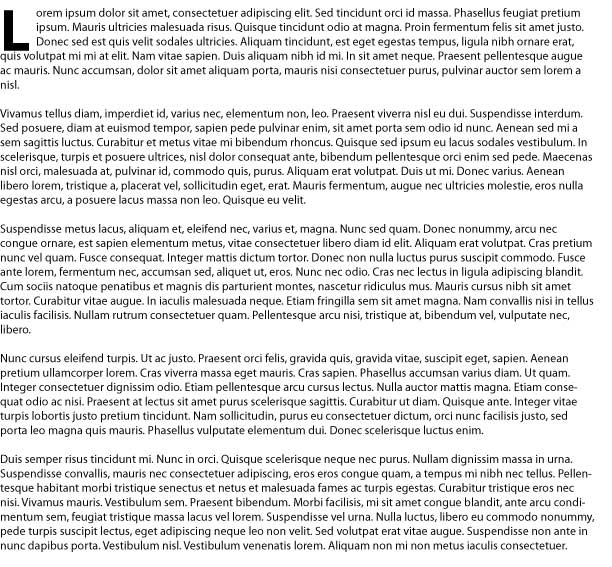
\includegraphics[width=\textwidth, height=\textheight]{imagenes/acta.jpg}

\setcounter{secnumdepth}{3}
\setcounter{tocdepth}{4}

% Define encabezado numeros romanos y como se separan los captiulos y las
% secciones
\addtolength{\headheight}{3pt}
\pagenumbering{roman}
\pagestyle{fancyplain}

\renewcommand{\chaptermark}[1]{\markboth{\chaptername\ \thechapter:\,\ #1}{}}
\renewcommand{\sectionmark}[1]{\markright{\thesection\,\ #1}}

\onehalfspacing

\lhead{}
\chead{}
\rhead{}
\renewcommand{\headrulewidth}{0.0pt}
\lfoot{}
\cfoot{\fancyplain{}{\thepage}}
\rfoot{}


% Pagina de resumen
\setcounter{page}{4}
\begin{center}
	{\bf Resumen} \pdfbookmark[0]{Resumen}{resumen} % Sets a PDF bookmark for the dedication
\end{center}	

EL CONTENIDO DEL RESUMEN.


% Pagina de dedicatoria (opcional)
\pagebreak

\setcounter{page}{5}

\vspace*{8cm} 
\pdfbookmark[0]{Dedicatoria}{dedicatoria} % Sets a PDF bookmark for the dedication
\begin{center} 
\large DEDICATORIA
\end{center}
\newpage


% Pagina de agradecimientos (opcional)
\setcounter{page}{6}

\chapter*{Agradecimientos
\markboth{Agradecimientos}{Agradecimientos}}
\pdfbookmark[0]{Agradecimientos}{agradecimientos}

\bigskip

AQU\'I VAN LOS AGRADECIMIENTOS.


% Crea la tabla de contenidos
\tableofcontents

% Crea la lista de cuadros
\listoftables

% Crea la lista de figuras
%\lstlistoflistings
\listoffigures

% Crea la lista de codigos fuentes

\clearpage

% Define encabezado en numeros arabicos  
\pagenumbering{arabic}

\fancyhf{} % Redefine el encabezado 
\lhead{}
\chead{}
\rhead{\fancyplain{}{\thepage}}
\renewcommand{\headrulewidth}{0.0pt}
\lfoot{}
\cfoot{}
\rfoot{}

\doublespacing

%\makeglossaries
% Incluye los archivos deseados - El contenido de su proyecto de grado/pasantia larga.
\chapter*{Introducción}

\pdfbookmark[0]{Introducción}{introduccion} % Sets a PDF bookmark for the dedication

\label{sect:motivacion}

AQU\'I VA EL CONTENIDO DE ANTECEDENTES. 

\label{sect:justificacion}

AQU\'I VA EL CONTENIDO DE LA JUSTIFICACI\'ON.

\label{sect:planteamiento}

AQU\'I VA EL CONTENIDO DEL PLANTEAMIENTO DEL PROBLEMA.

\label{sect:objetivo_general}

AQU\'I VA EL OBJETIVO GENERAL.

\label{sect:objetivos_especificos}

AQU\'I VAN LOS OBJETIVOS ESPEC\'IFICOS.


% Marco Teorico.
\chapter{Marco teórico} \label{chap:marco_teorico}

AQU\'I VA EL CONTENIDO DEL MARCO TE\'ORICO.

Los conceptos m'as importantes sobre ...

La secci'on \ref{sect:procesos} presenta las definiciones b'asicas para
entender ...


\section{Procesos} \label{sect:procesos}

Para explicar el uso del ...

Referencia a uno de los libros \cite{S09}.


\chapter{Presentación del problema}\label{chapter:presentacion_del_problema}

AQU\'I VA EL DESARROLLO DEL PLANTEAMIENTO DEL PROBLEMA.

Los requerimientos de la herramienta o software a implementar se mencionan a
continuaci'on: 

\label{sect:objetivos}
Mientras que como objetivos parciales o específicos se postulan los siguientes:
\begin{itemize}
\item {Diseñar y elaborar ...}
\end{itemize}

\chapter{Resultados}\label{chapter:resultados}

AQUI VA EL CONTENIDO DE RESULTADOS.
	
\textbf{C'odigo de ejemplo:}
\begin{figure}[h]
\begin{lstlisting}[mathescape]
for x in $\sim$ :
  pass
\end{lstlisting}
\caption[Ejemplo c'odigo]
{Ejemplo c'odigo}
\label{ejemplo_codigo}
\end{figure}

As'i referencias una figura \ref{ejemplo_codigo}.

Una lista de cosas:
\begin{itemize}
 \item {Objeto 1.} 
 \item {Objeto 2.} 
\end{itemize}

\begin{figure}[h]
	\begin{center}
		
\includegraphics[scale=0.4]{imagenes/cebolla.png}
	\end{center}
	\caption{
		\label{fig:cebolla}
		Logo USB
	}
\end{figure}

As'i referencias una imagen \ref{fig:cebolla}.

\begin{table}[h]
\centering
\begin{tabular}{|c|c|}
\hline
T'itulo 1 & T'itulo 2 \\
\hline
Objeto 1 & Objeto 2 \\
\hline
Objeto 3 & Objeto 4 \\
\hline
\end{tabular}
\caption{Table de ejemplo}\label{tab:tabla_ejemplo}
\end{table}

\begin{teorema} \label{teo:formula}
Si $\{X(t) \text{, } 0 < t < \infty \}$ es un proceso as-H
\end{teorema}

\begin{equation} \label{eq:tipoestacionarios1}
Y(t) = e^{-tH}X(e^t) \text{, } - \infty < t < \infty
\end{equation}


\chapter{Conclusiones y recomendaciones} 

\label{chap:conclusiones}

Logrando los objetivos ...


% Establece las citas y bibliografia
\bibliographystyle{alpha.bst}
\bibliography{myrefs}

% Crea el apendice
\appendix
\chapter{Archivos intermedios}

%---------------------------------------------------------------------------------------%
\section {Representación de Dominio}

\label{archivos_intermedios:dom}
El archivo contiene los valores posibles ....

\chapter{Gram'atica del Lenguaje}

%---------------------------------------------------------------------------------------%
\section {Representación de Dominio}

El archivo por ejemplo para el nodo ...


\chapter*{Glosario}

\pdfbookmark[0]{Glosario}{glosario}

\subsection*{Aleatorio}
Indica la condición de que una acción produzca resultados con un cierto grado de azar. En la computación el concepto ``aleatorio'' es utópico y por ende, en su lugar se utiliza la palabra ``pseudoaleatorio'' que indica que el resultado no es totalemnte al azar. 7

\subsection*{Grafo}
Es una estructura de datos que representa la forma en la que muchos entes denominados ``nodos'' estan relacionados entre si por valores o condiciones específicas llamados ``arcos''. 9


\end{document}
